% Lab 4: WEKA and Data
% Author: Rob Kelly
%
% CSE/IT 489/589-06: Introduction to Neural Network Applications
% Spring 2016
% New Mexico Tech
%
% Lab Goal: (spooky skeleton)
% \_ Cleaning Bad Data
% \_ Feature Selection
% \_ Encoding
% \_ PCA (SCRAPPED, three sections is enough for a 1-hour lab)
%
% Side note: Parts of this lab were adapted from an assignment from a class at
% George Mason University taught by Dr. Huzefa Rangwala. This includes the
% MNIST handwriting dataset ARFF file, and the rendered images of the data.
% These were sourced from http://cs.gmu.edu/~hrangwal/files/a1/ on 2016/4/13.
%

\documentclass[11pt]{cselabheader}

\usepackage{enumitem}

\fancyhead[R]{Lab 4: WEKA and Data}
\title{Neural Network Applications -- Lab 4 \\ WEKA and Data\footnote{The ARFF dataset of the MNIST handwriting samples used in this lab was adapted from a class taught by H. Rangwala at George Mason University.}}

\begin{document}
\maketitle

\horrule{0.5pt}\\\horrule{2pt}

\section{Background}

% This lab activity will serve as an introduction to using backpropagation-trained neural networks in WEKA. WEKA ships with the Multilayer Perceptron classifier, a feed-forward neural network architecture with hidden layers trained using backpropagation. Neural network algorithms with one or more hidden layers -- layers other than the input or output -- are sometimes called \emph{deep learning} algorithms, and are useful for learning complicated behaviors in data which aren't well-understood. For this reason, there's been a great deal of renewed interest in the Multilayer Perceptron architecture in the past few years.

% It should be noted that the name ``Multilayer Perceptron'' is something of a misnomer. This algorithm has only a tenuous connection to the Perceptron learning algorithm. A multilayer Perceptron network is not a Perceptron, nor are the individual neurons of the network Perceptron neurons -- a multilayer Perceptron uses the sigmoid activation function. Despite this, the name has stuck, and is abundant in the literature.

In past lab exercises, we've followed a set pattern: take a dataset, pick a classifier, train and evaluate. Much of our study has focused on optimizing parameters to this classifier. In practice, things are rarely so simple. Not all data is perfectly suited for every model; a large degree of the work of a data scientist is \emph{processing} the data, \emph{filtering out} bad data points, \emph{analyzing} the information underlying the data, and \emph{encoding} the data for classification.

WEKA provides us with a useful set of tools for data processing and analysis, and this lab exercise will introduce a number of them. In this lab, we'll be examining the MNIST handwriting dataset. This set consists of about 2000 images of handwritten numerals, and is fairly well-known in neural-network pedagogy.

\begin{figure}[h]
  \centering
  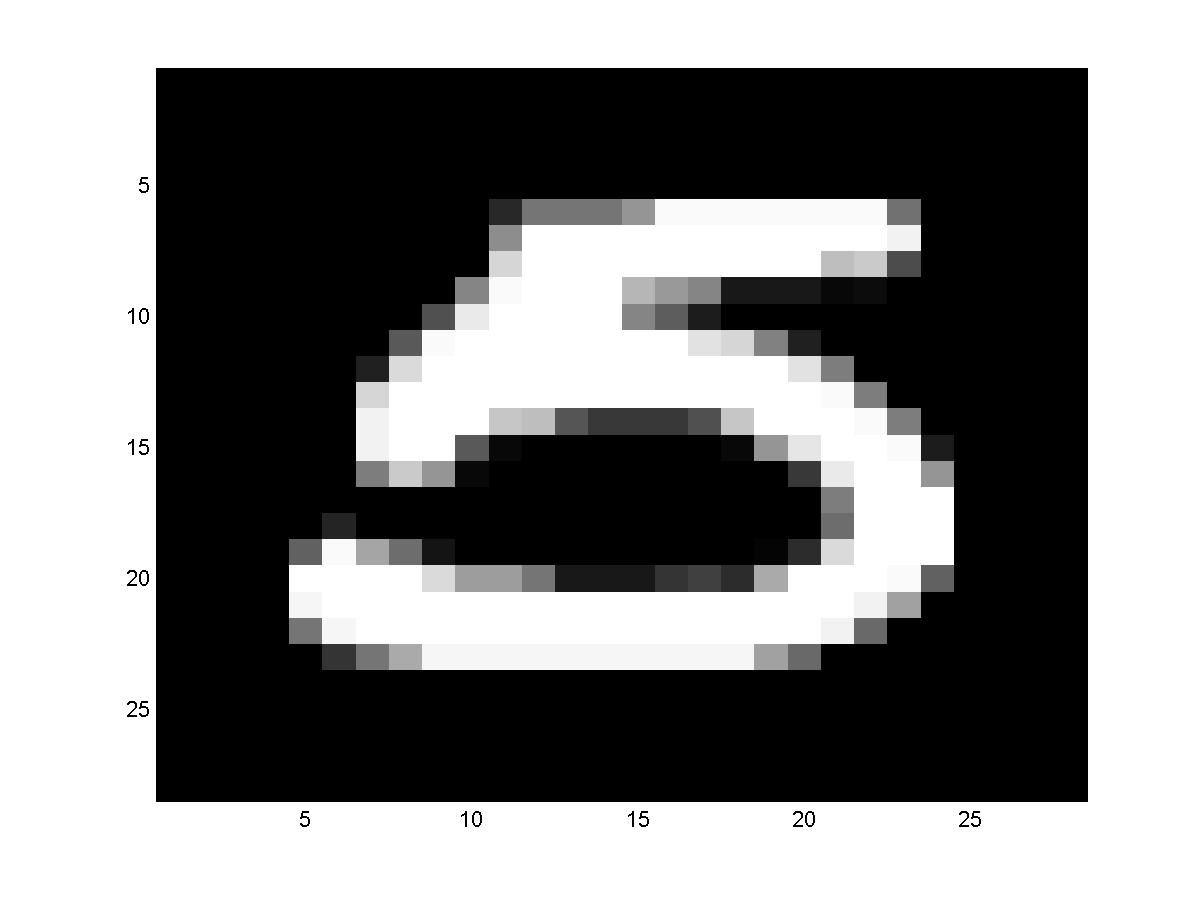
\includegraphics[width=0.2\textwidth]{mnist_5.png}
  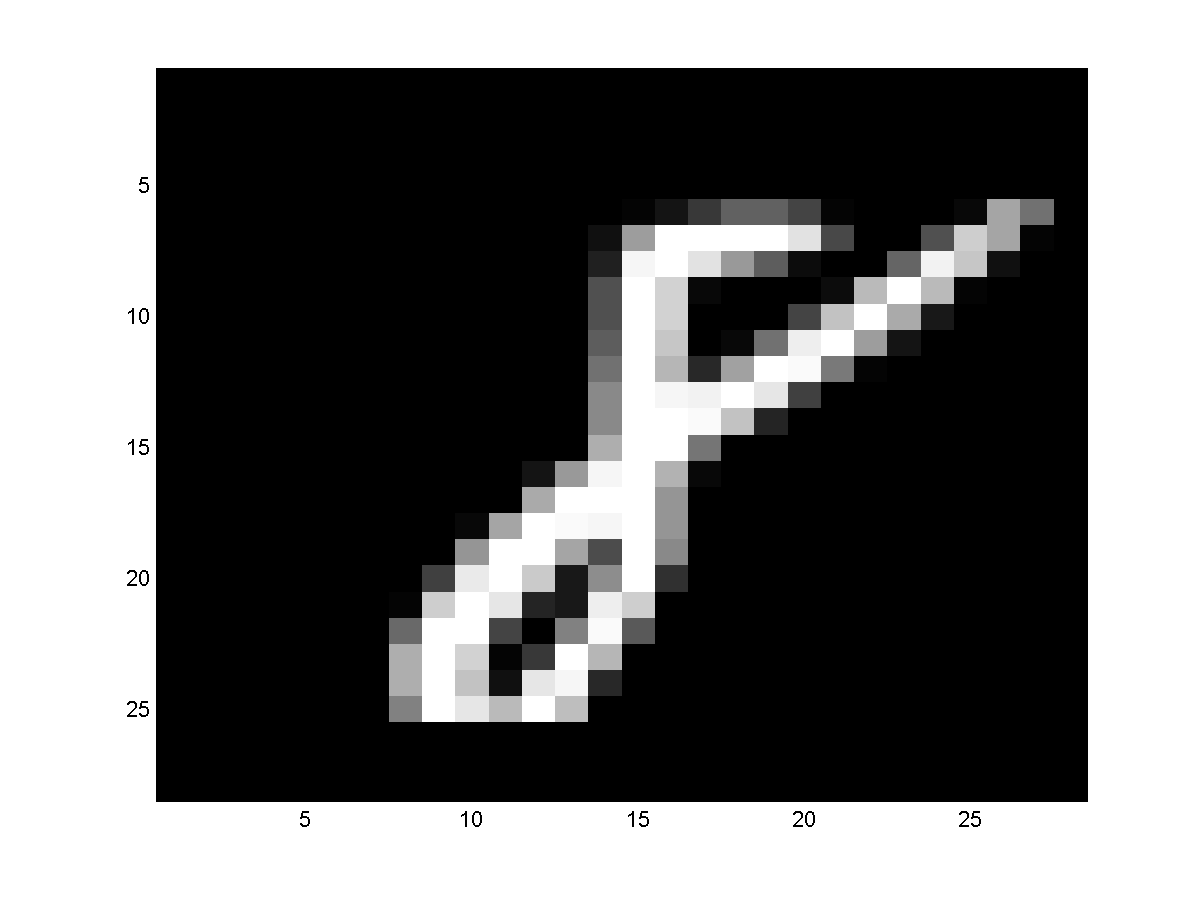
\includegraphics[width=0.2\textwidth]{mnist_8.png}
  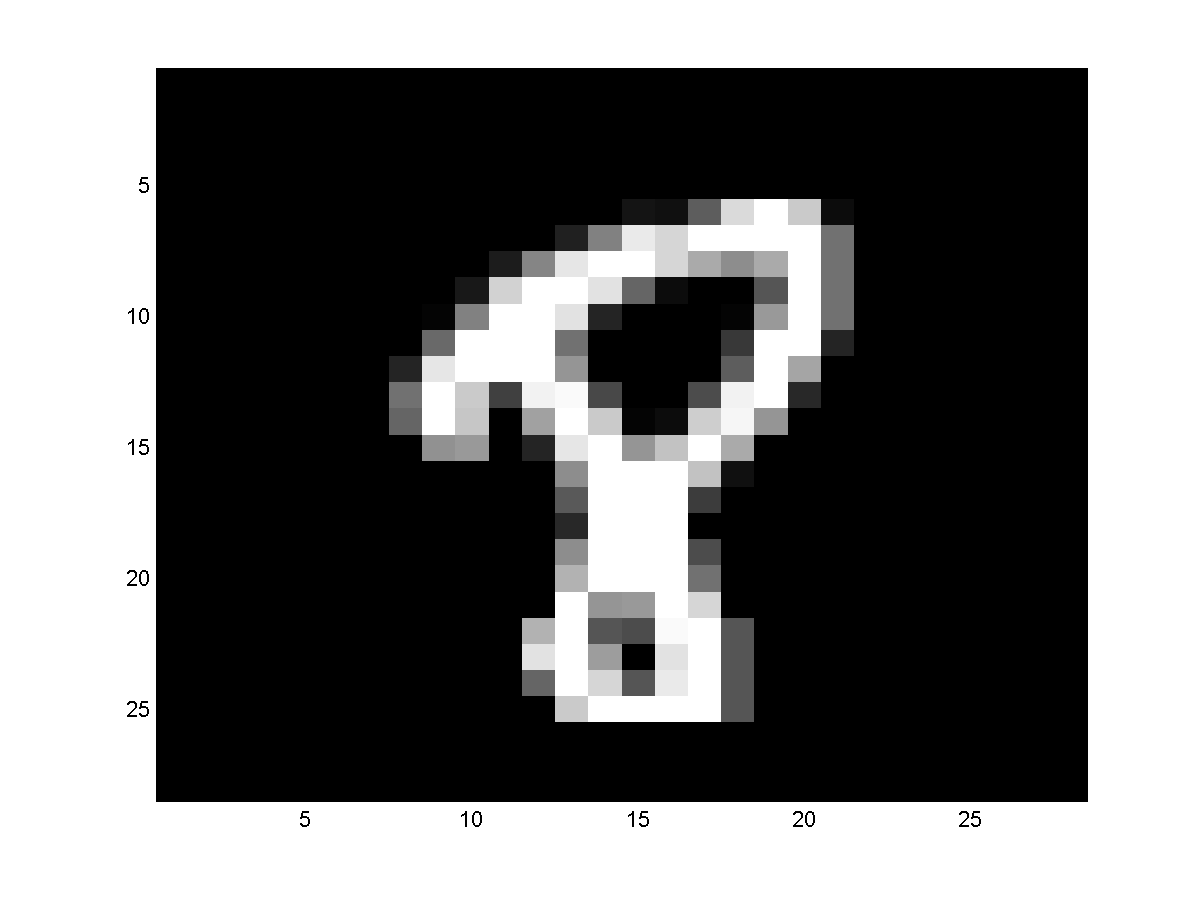
\includegraphics[width=0.2\textwidth]{mnist_8_2.png}
  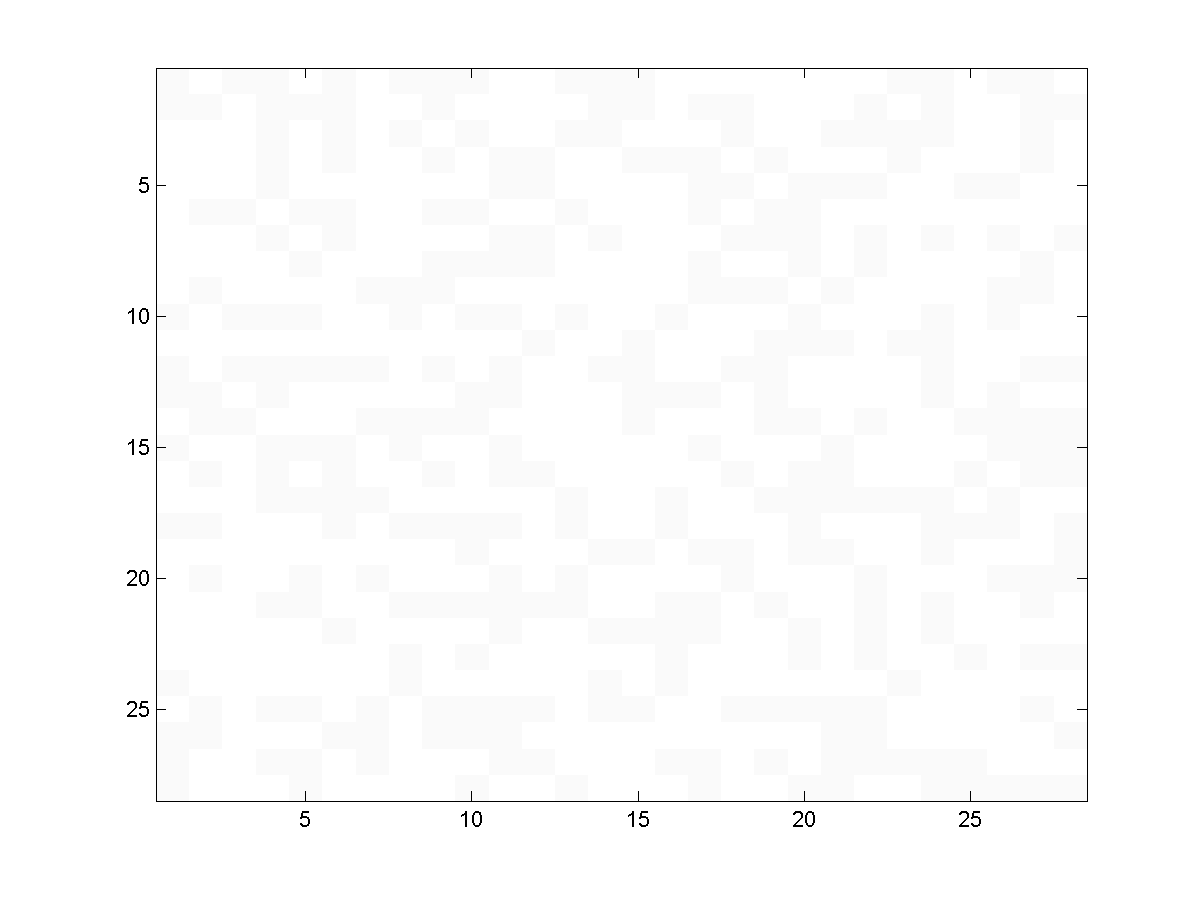
\includegraphics[width=0.2\textwidth]{mnist_bad.png}
  \caption{Four images from our MNIST handwriting dataset.}
\end{figure}

These images are encoded as $28 \times 28$-pixel grayscale bitmaps; in the dataset, each instance is a vector of 784 numeric pixel values ranging from 0 to 255, with an additional nominal class attribute denoting the digit 0-9. The dataset has been provided as an ARFF on the assignment page. Also included is an archive of PNG renderings of the data -- it may be useful to cross-reference these with the dataset. Note that this dataset includes a few ``bad'' error instances, so we'll need to do something about those as well...

\pagebreak

\section{Lab Exercises}

\subsection{Cleaning Bad Data}
\begin{itemize}[leftmargin=*]
  \item Open \texttt{mnist.arff} in the WEKA explorer. This dataset will be included on the Canvas page for this lab.

  \item Let's get a baseline for performance before we do anything else. Train a \textsc{lvq3} classifier on the dataset and evaluate with 10-fold cross-validation. Leave all the parameters as default. Save the result buffer; you will be submitting it later.

  \item Open the \emph{Preprocess} tab. Select any attribute of the dataset to visualize it as a histogram in the lower left. Likewise, open the \emph{Visualize} tab. This view shows a plot of each attribute against every other, with each point representing an instance, indicating class by color. Click on any of these plots to enlarge. Many of these points will overlap; use the \emph{jitter} slider to ``spread them out'' a bit. You can view the details of any specific point by clicking on it.
 
  \begin{ex}\label{ex1}
    We know that the dataset includes ``bad'' noisy images. Looking through the visualization plots, do you notice anything unusual?
  \end{ex}

  \item Use WEKA to clean up the data based on the observations you made in Exercise~\ref{ex1}. In the \emph{Preprocess} tab, use the \emph{RemoveWithValues} filter (under \texttt{weka.filters.unsupervised.instance}) to remove instances from the dataset based on the value of some given attribute(s). The ``More'' button on the parameters panel will tell you how to use this filter.

  \item Save the ``cleaned'' dataset somewhere -- you'll be doing this a few times during this lab exercise.

  \item Train and evaluate a \textsc{lvq3} classifier with the same parameters you used before, and again save the result buffer.

  \begin{ex}
    Did the performance of the classifier improve when bad data was removed? Think about how the model is evaluated -- does this change in evaluated performance tell us anything about how the model would perform in a real-world application?
  \end{ex}
\end{itemize}

\subsection{Feature Extraction}
\begin{itemize}[leftmargin=*]
  \item Now we're going to look at removing attributes of the data which don't provide useful information to our model. Look through the histograms of a few attributes in the \emph{Preprocess} tab. Use the \emph{RemoveUseless} filter (under \texttt{weka.filters.unsupervised.attribute}) to remove any useless attributes. Check the documentation as before to learn how to use this.

  \begin{ex}
    We're describing these attributes as ``useless.'' With respect to our task (classification), what do we mean by this, and why are these attributes useless?
  \end{ex}

  \item We've removed the totally useless attributes, so now we can move our focus to attributes which are simply \emph{less useful}. Open the \emph{Select Attributes} tab, choose the \emph{InfoGainAttributeEval} attribute evaluator, and run it. This ranks the attributes of the data set by information gain.
  \begin{itemize}[leftmargin=*]
    \item \textit{Notice that the \emph{Ranker} search method is chosen automatically -- it's the only method relevant to this attribute evaluator.}
  \end{itemize}

  \begin{ex}
    What does ``information gain'' mean here? Support your answer by looking at the histograms and scatter-plots of high-info-gain and low-info-gain attributes. Also, check the \emph{InfoGainAttributeEval} for a formal definition.
  \end{ex}

  \item We can apply this ranking to the dataset using a preprocessing filter. In the \emph{Preprocess} tab, choose the \emph{AttributeSelection} filter (under \texttt{weka.filters.supervised.attribute}). Set the \texttt{evaluator} to \emph{InfoGainAttributeEval} and the \emph{search} method to \emph{Ranker}. Apply this.

  \item Use the \emph{Remove} filter to remove all the attributes with zero information gain by specifying a range of attributes to remove.
  \begin{itemize}[leftmargin=*]
    \item \textit{Since the attributes are now in ranked order, these would be the ones at the bottom.}
    \item \textit{\textbf{Don't} remove the class attribute.}
  \end{itemize}

  \item Save the filtered dataset. Don't overwrite the cleaned dataset you saved earlier.

  \item Train and evaluate a \textsc{lvq3} classifier as before and save the results.

  \begin{ex}
    Compare the performance of this classifier to that of the previous section. Why did removing these particular attributes affect the performance of the model?
  \end{ex}

  \begin{ex}
    At the start of this exercise, our dataset had 785 attributes; now it has 525. We could reduce the dimensionality of our data even further if we wished. Often, dimensionality reduction comes at the cost of some degree of information loss.

    Why might we want to use data with fewer dimensions? There are many correct answers, but more specifically, why would we want lower-dimensionality data for a model trained with \emph{backpropagation}?
  \end{ex}
\end{itemize}

\subsection{Encoding}
\begin{itemize}[leftmargin=*]
  \item All of the attributes of the data are currently numeric, representing grayscale pixel values on a scale of 0.0 (black) to 255 (white). In the \emph{Preprocess} tab, use the \emph{NumericToBinary} filter (under \texttt{weka.filters.unsupervised.attribute}) to convert all attributes but the class to unipolar binary encoding.

  \item Again, save the binary-encoded dataset, and train and evaluate the classifier and save the results.

  \begin{ex}
    Like before, compare the performance of this classifier to that of the previous section. Why did this change of encoding affect the performance of the model?
  \end{ex}

\end{itemize}

% \subsection{Principal Component Analysis}
% \begin{itemize}[leftmargin=*]
%   \item 
% \end{itemize}

\pagebreak

\section{Submitting}

You will be submitting the following files:

\begin{itemize}
  \item A PDF or plaintext document containing your solutions to exercises 2.1 -- 2.7.
  \item Your cleaned, filtered, and binary-encoded datasets as three different ARFF files.
  \item Your four classifier result buffers: the preliminary evaluation, and the ones created at the end of each section.
\end{itemize}

 This lab is to be submitted as a group; submit a \texttt{tar} archive named \texttt{group\_\#\_lab4.tar.gz} (where \# denotes your group's number) on the \emph{Lab 4} assignment section on the course Canvas page.

\end{document}